\section{Introduction}\label{introduction}

\begin{frame}{Path finding as decision problems}

\begin{figure}
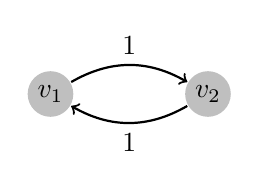
\begin{tikzpicture}[->,line join=bevel, thick]
  \tikzstyle{vertex}=[circle,fill=black!25,minimum size=12pt,inner sep=2pt]
  \node[vertex] (G_1) at (-2,0)  {$v_1$};
  \node[vertex] (G_2) at (0,0)   {$v_2$};
  \path (G_1) edge [bend left] node[above] {1} (G_2)
        (G_2) edge [bend left] node[below] {1} (G_1);
\end{tikzpicture}
\caption{A simply cyclic markov chain. For a definition of the term cyclic we refer to appropriate literature.}
\label{cyclic-graph}
\end{figure}

\begin{itemize}
\item
  Example graphs + animation
\item
  Interesting result: UPATH \emph{seems} to be easier (note: PATH
  \emph{could} be just as easy if $L = NL$)
\end{itemize}

\end{frame}

\begin{frame}{Random Walk}

\begin{itemize}
\itemsep1pt\parskip0pt\parsep0pt
\item
  Example animation (dice as random visualization)
\end{itemize}

\end{frame}

\begin{frame}{Universal Traversal Sequence}

\begin{itemize}
\itemsep1pt\parskip0pt\parsep0pt
\item
  Example for graph of size 3 with d=2 (there are only 3)
\end{itemize}

\end{frame}

\section{Space-Complexity}\label{space-complexity}

Foo

\begin{frame}{Definition}

\begin{itemize}
\itemsep1pt\parskip0pt\parsep0pt
\item
  Turing machine model (picture)
\end{itemize}

\end{frame}

\begin{frame}{Examples}

\begin{itemize}
\itemsep1pt\parskip0pt\parsep0pt
\item
  What can we do with poly/log/constant space
\end{itemize}

\end{frame}

\begin{frame}{$NLSPACE \subseteq P$}

\begin{itemize}
\itemsep1pt\parskip0pt\parsep0pt
\item
  Proof
\end{itemize}

\end{frame}

\begin{frame}{PATH is NL-complete}

\begin{itemize}
\itemsep1pt\parskip0pt\parsep0pt
\item
  Informal definition of NL-completeness:

  \begin{itemize}
  \itemsep1pt\parskip0pt\parsep0pt
  \item
    Transform instance of decision problem A to instance for B and use B
    to solve it
  \item
    Restrict power of transformation function
  \end{itemize}
\item
  More precisely cover the transformation: TM -\textgreater{}
  configuration graph

  \begin{itemize}
  \itemsep1pt\parskip0pt\parsep0pt
  \item
    only log-bounded space needed to encode current configuration
  \item
    look at possible next configurations and write to output tape
  \end{itemize}
\item
  Applying PATH to that should be trivial
\end{itemize}

\end{frame}

\section{RL and RandomWalk}\label{rl-and-randomwalk}

\begin{itemize}
\item
  Use RandomWalk to construct randomized decider for $UPATH$
\item
  Show that it can not work for $PATH$
\end{itemize}

\begin{frame}{Proofing a bound on the number of steps}

\begin{itemize}
\item
  Short example of Markov-Chain
\item
  Relation to RandomWalk: Important connected graph
\item
  RandomWalk can be modeled as Markov-Chain (Markov Property)
\item
  Derive expected length of a random walk starting at any node $a$ to
  reach any other node $b$: We proof an upper bound: Expected number of
  steps to visit all nodes in G.
\item
  Overview:
\item
  First compute $P_v$ and thus $E(v, v)$
\item
  Compute upper bound for $E(u, v)$
\item
  Compute upper bound for $E(a, G)$
\item
  Apply Markov-Inequality to compute probaboility that we need more than
  8\emph{e}n steps.
\end{itemize}

\end{frame}

\section{Universal Traversal
Sequences}\label{universal-traversal-sequences}

\begin{frame}{d-regular graphs}

\begin{itemize}
\itemsep1pt\parskip0pt\parsep0pt
\item
  Definition
\item
  Number of d-regular graphs of size n
\item
  Traversal sequences and random walks
\end{itemize}

\end{frame}

\begin{frame}{Probability amplification}

\begin{itemize}
\itemsep1pt\parskip0pt\parsep0pt
\item
  Conduct $m$ random walks, probability of not finding a path is
  $2^{-m}$, but size only $8en \cdot m$
\item
  Make $m$ big enough that the probability of a given traversal
  sequences to work for all graphs is bigger than 0:

  \begin{itemize}
  \itemsep1pt\parskip0pt\parsep0pt
  \item
    Again markov inequality: $E(F) = g_{n, d} \cdot 2^{-m} < 1$, thus:
    $1 - Pr[F < 1] = Pr[F \geq 1] \leq E(F) / 1$ \textless{} 1 which
    results in $0 < Pr[F < 1]$
  \end{itemize}
\end{itemize}

\end{frame}
